\vspace{-1em}
\section{RESULTS}\label{sec:results}
\vspace{-0.25em}
Tests on the synthetic data were in the range of 86-95\% correct detection
(Table \ref{tab:synthtests}). The method
achieved the highest accuracy in the \textbf{bidrop} shape, and the lowest in
the \textbf{drop} shape.
\begin{table}[hbpt]
\centering
  \caption{\small
  Number of corners detected per shape. The accuracy of the method
  is highlighted.}
  \begin{tabular}{r|ccccc}
\hline
Shapes / & \multicolumn{5}{c}{Number of corners detected (\%)}\\
Corners & None & 1 & 2 & 3 & $\geq 4$\\
\hline
Circle  & \textbf{89.35} & 0 & 0 & 0.47  & 10.18\\
Drop & 4.42 & \textbf{86.02}  &  6.81 &   2.52  &   0.23\\
Bidrop & 0 & 0.41  &  \textbf{95.17}  &   4.31  &  0.11\\
Tridrop   & 0  &  0.02  &  2.76  &   \textbf{92.94}  &   4.28\\
\hline
  \end{tabular}
  \label{tab:synthtests}
\end{table}
Figure \ref{fig:res-all} displays the shape evolution of a track-fragment containing 50
frames in the dataset. Eight frames are shown with the moved boundary displayed in the
dotted line (cyan- -) and the evolved shape in the solid line (magenta-) (Top row). 
For visual assessment, the corners detected by the anglegram at each point are
displayed as asterisks (yellow$*$).
% Corners
% detected by the anglegram at each point are also displayed as asterisks (yellow$*$)
% for visual assessment.
The orientation and aspect ratio are plot together (middle row), and
the number of corners and the measured angle (bottom row).
\begin{figure*}[hbpt]
    \centering
    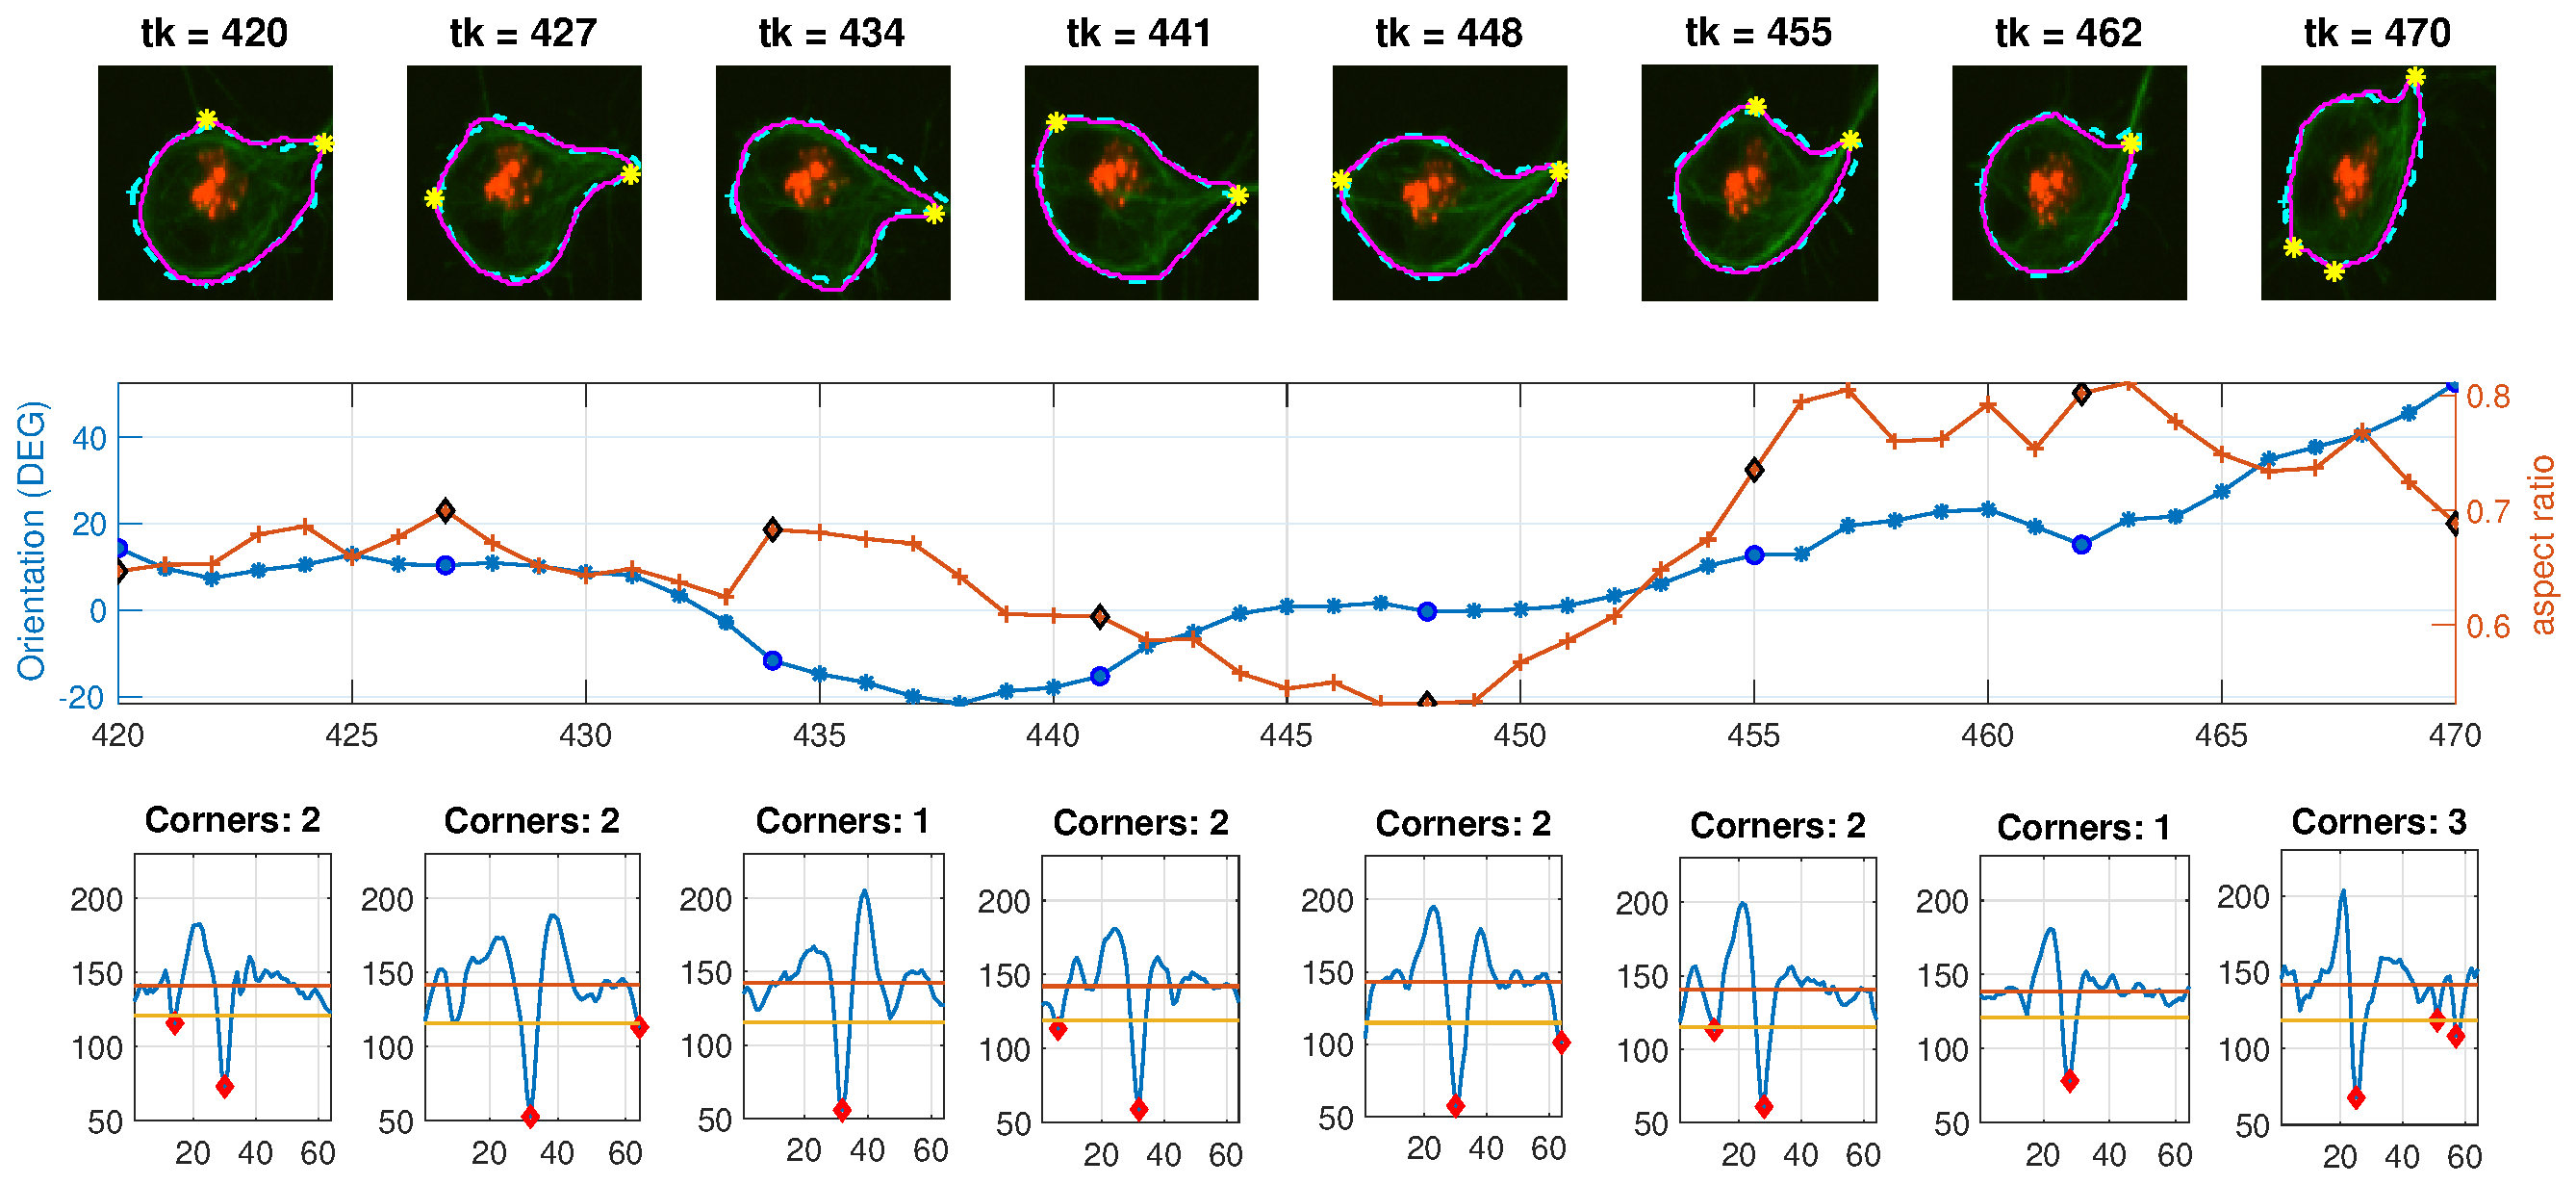
\includegraphics[width=0.9\textwidth, height=0.25\textheight]{mat-fig8}
    \caption[Evolution of a cell shape]{\small
    Evolution of cell shape throughout multiple frames. \textbf{Top row}:
    Eight instances of 50 consecutive frames. Previous segmentation in
    cyan(- -),
    evolved in magenta(-) and corners detected in yellow($*$).
    \textbf{Middle row}: Comparison between the orientation (blue $*-$) and
    the aspect ratio (orange $+-$). The values for the \textbf{top} frames
    are highlighted in blue($\circ$) and black ($\diamond$).
    \textbf{Bottom row}: Minimum intensity projection of \textbf{top}'s'
    respective anglegrams displaying the values of the angles measured
    per corner (red $\diamond$).
    }
    \label{fig:res-all}
\end{figure*}
